
\subsection{Fit Procedure}
\label{sec:fit}

A maximum-likelihood fit is performed over the total yields in the various fit regions described in Section \ref{sec:evt_selection} in order to extract the best-fit value of the WZ + b-jet and WZ + charm jet contributions for events with both 1 and 2 associated jets.

Because the fit regions are defined by the number of associated jets at reco-level, the signal is split into separate samples based on the number of truth jets in order to account for differences in the number of truth jets compared to the number of reco-jets. The $WZ$ + b, $WZ$ + charm and $WZ$ + light contributions are separated into independent samples based on the number of truth jets in each event. WZ + 1 truth-jet and WZ + 2 truth-jets are treated as signal samples, while WZ + 0 truth-jets and WZ + $>=$3 truth-jets are treated as an additional background. 

A maximum likelihood fit to data is performed simultaneously in the regions described in Section \ref{sec:evt_selection}, summarized in figure \ref{fig:summary}. The six signal templates, which include WZ+b 1-jet, WZ+c 1-jet, WZ+l 1-jet, WZ+b 2-jets, WZ+c 2-jets, WZ+l 2-jets, are allowed to float, while the remaining background contributions are held fixed. The parameters $\mu_{WZ+b - 1-jet}$, $\mu_{WZ+charm 1-jet}$, $\mu_{WZ+light - 1-jet}$, $\mu_{WZ+b - 2-jet}$, $\mu_{WZ+charm 2-jet}$, $\mu_{WZ+light - 2-jet}$, where $\mu = \sigma_{observed}/\sigma_{SM} $, are extracted from the fit. A simultaneous fit is performed over all 1-jet and 2-jet regions.

\begin{figure}[H]
  \center                                                                                                                    
  \includegraphics[width=.9\linewidth]{sys_truthJets/Plots/Summary_postFit.png}
  \caption{Post-fit summary of the fit regions.}
  \label{fig:summary}
\end{figure}

As described in Section \ref{sec:sys}, there are 230 systematic uncertainties that are considered as NPs in the fit. These NPs are constrained by Gaussian or log-normal probability density functions. The latter are used for normalisation factors to ensure that they are always positive. The expected number of signal and background events are functions of the likelihood. The prior for each NP is added as a penalty term, decreasing the likelihood as it is shifted away from its nominal value.

Several alternate fit strategies are documented in Appendices \ref{sec:incFit}-\ref{sec:inc_tZ}. These include a measurement of WZ + 1 or 2 jets inclusively, a fit where tZ is allowed to float, and a case where tZ is included as part of the signal.

\subsection{Fiducial Region Definition}
\label{sec:fid}

The fiducial volume at particle level is defined based on the number of stable leptons and jets in each event. Three light leptons with total charge $\pm$1 and one or two associated jets are required. This is separated into four observations based on the number and flavor of associated jets.

Only leptons which do not originate from hadron or $\tau$ decays are considered. The phase space definitions use dressed kinematics of the final state particles. Leptons are dressed by summing the momentum of photons within a cone of $\Delta R < 0.1$ of the lepton to correct the leptons energy. Particle level jets are reconstructed using the anti-$k_t$ algorithm with a radius of $R=0.4$. 

The kinematic selection used at particle level closely follows the selection used at reconstructed level. Three light leptons with total charge $\pm$1 and one or two associated jets  Leptons and jets are required to have $|\eta| < 2.5$, with the transition region included. The OS leptons is required to have $p_T > 10$ GeV, while the SS leptons are required to have $p_T > 20$ GeV. Jets are required to have $p_T > 25$ GeV. The base fiducial region definition is summarized below:

\begin{itemize}
\item Three light leptons with total charge $\pm$1, $|\eta| < 2.5$
\item OS lepton with \pt$>$10 GeV, SS leptons with \pt$>$20 GeV
\item One OSSF lepton pair with $|M(ll)-91.2\ GeV| < 10\ GeV$
\item One or two associated truth jets with $p_T >$25 GeV, $|\eta| < 2.5$
%\item At least one truth b-jet or one charm jet
\end{itemize}

The result of the fit is used to extract the cross-section in this fiducial region for WZ + b and WZ + charm with one associated jet, and WZ + b and WZ + charm with two associated jets, where the number and flavor of the jets is determined at particle level. Events with both charm and b-jets are counted as WZ + b.

\subsection{Results of the Simultaneous Fit}
\label{sec:resSum}

The Asimov fit for 1-jet events gives an expected $\mu$ value of $1.00^{+0.47}_{-0.43}(stat)^{+0.30}_{-0.27}(sys)$ for $WZ$ + b. The fitted cross-section modifiers for $WZ$ + charm and $WZ$ + light are $1.00 \pm 0.17 \pm 0.17$ and $1.00 \pm 0.06 \pm 0.14 $, respectively.

\hspace{-1in}\begin{table}[H]
\begin{adjustwidth}{-3em}{-3em}
\begin{center}
\begin{tabular}{l|cc}
\hline
Process & $\mu$ & $\sigma$ \\
WZ + b - 1-jet & $1.00^{+0.47}_{-0.43}(stat)^{+0.30}_{-0.27}(sys)$ & \\
WZ + c - 1-jet & $1.00 \pm 0.17(stat) \pm 0.17(sys)$ & \\
WZ + b - 2-jet & $1.00^{+0.53}_{-0.51}(stat)^{+0.39}_{-0.34}(sys)$ & \\
WZ + c - 2-jet & $1.00 \pm 0.25(stat) \pm 0.21(sys)$ & \\
\hline
\end{tabular}
\caption{Correlations between the various components of WZ}
\label{tab:WZ_res }
\end{center}
\end{adjustwidth}
\end{table}

The expected cross-section of WZ+b with 1-jet is $1.74^{+0.82}_{-0.75}(stat)^{+0.53}_{-0.48}(sys)$ fb, and $14.6 \pm 2.5 (stat) \pm 2.3 (sys)$ fb for WZ + charm, with a correlation of -0.15 between them. An expected significance of 2.0 is observed for WZ + b in this region. 

For 2-jet events, the fit gives an expected $\mu$ value of $1.00^{+0.53}_{-0.51}(stat)^{+0.39}_{-0.34}(sys)$ for $WZ$ + b. The fitted cross-section modifiers for $WZ$ + charm and $WZ$ + light are $1.00 \pm 0.25 \pm 0.21$ and $1.00 \pm 0.06 \pm 0.16 $, respectively.

The expected $WZ$ + b cross-section in the 2-jet region is $2.5^{+1.3}_{-1.3}(stat)^{+0.95}_{-0.83}(sys)$ fb with an expected significance of 1.7$\sigma$. The 2-jet expected cross-section of $WZ$ + charm is $12.7 \pm 3.2 (stat) \pm 2.7 (sys)$ fb, and the correlation between WZ + charm and WZ + b is -0.22. 

A summary of the correlation between the various WZ components is summarized in Table \ref{tab:WZ_corr}.

\hspace{-1in}\begin{table}[H]
\begin{adjustwidth}{-3em}{-3em}
\begin{center}
\begin{tabular}{l|cccccc}
\hline
 & WZ + b - 1-jet & WZ + c - 1-jet & WZ + l - 1-jet & WZ + b - 2-jet & WZ + c - 2-jet & WZ + l - 2-jet\\
WZ + b - 1-jet & 1.00 & -0.15 & 0.28 & -0.13 & -0.22 & 0.17 \\
WZ + c - 1-jet & - & 1.00 & 0.36 & 0.13 & -0.14 & -0.16 \\
WZ + l - 1-jet & - & - & 1.00 & 0.10 & -0.20 & -0.39 \\
WZ + b - 2-jet & - & - & - & 1.00 & -0.22 & 0.17 \\
WZ + c - 2-jet & - & - & - & - & 1.00 & 0.23 \\
WZ + l - 2-jet & - & - & - & - & - & 1.00 \\
\hline
\end{tabular}
\caption{Correlations between the various components of WZ}
\label{tab:WZ_corr}
\end{center}
\end{adjustwidth}
\end{table}

The impact of each NP is calculated by performing the fit with the parameter of interest held fixed, varied from its fitted value by its uncertainty, and calculating $\Delta\mu$ relative to the baseline fit.  The impact of the most significant sources of systematic uncertainties on WZ + b with one associated jet is summarized in Table \ref{tab:systematics_1j}. 

\begin{table}[H]
    \centering
    \begin{tabular}{l|cc}
        \hline\hline
        Uncertainty Source & \multicolumn{2}{c}{$\Delta \sigma/\sigma_{nominal}$ }  \\
        \hline
        WZ + 1-jet light cross-section & 0.13 & -0.15 \\
        WZ + 1-jet charm cross-section & -0.10 & 0.12 \\
        Jet Energy Scale & 0.1 & -0.13 \\
        Other Diboson + b cross-section & -0.09 & 0.09 \\
        tZ cross-section & -0.08 & 0.08 \\
        WZ 1-jet/2-jet Migration & 0.08 & -0.07 \\
        Jet Energy Resolution & -0.07 & 0.08 \\
        Luminosity & -0.06 & 0.07 \\
        Flavor tagging & 0.05 & 0.05 \\
        $t\bar{t}$ cross-section & -0.05 & 0.05 \\
        \hline
        Total Systematic Uncertainty & 0.28 & 0.33 \\
        \hline\hline
    \end{tabular}
    \caption{Summary of the most significant sources of systematic uncertainty on the measurement of $WZ+b$ with exactly one associated jet.}
    \label{tab:systematics_1j}
\end{table}

The ranking and impact of those nuisance parameters with the largest contribution to the overall uncertainty is shown in Figure \ref{fig:ranking_1j}.

\begin{figure}[H]
    \centering
    \includegraphics[width=0.7\linewidth]{sys_truthJets/Ranking.png}
    \caption{Impact of systematic uncertainties on the signal-strength of $WZ$ + b for events with exactly one jet}
    \label{fig:ranking_1j}
\end{figure}

The large impact of the Jet Energy Scale and Jet Flavor Tagging is unsurprising, as the shape of the fit regions depends heavily on the modeling of the jets. The other major sources of uncertainty come from background modelling and cross-section uncertainty. %The pie charts in Figure \ref{fig:pie_chart_1j} show that for the modelling uncertainties that contribute most correspond to the most significant backgrounds. 

%The negative correlations between $\mu_{WZ+charm}$ and $\mu_{WZ+b}$ and $\mu_{WZ+light}$ are expected: $WZ$ + charm is present in both the $WZ$ + b and $WZ$ + light enriched regions, therefore increasing the fraction of charm requires increasing the fraction of $WZ$ + b and $WZ$ + light. This reasoning also explains the positive correlation between $\mu_{WZ+b}$ and $\mu_{WZ+light}$. 

%Two of the major backgrounds in the region with the highest purity of $WZ$ + b are tZ and Other VV + b, explaining the negative correlations between $\mu_{WZ+b}$ and the tZ cross section, and the VV + b cross section.

%The high correlation between the luminosity and $\mu_{WZ+light}$ arises from the fact that the uncertainty on $\mu_{WZ+light}$ is very low (around 4\%). Small changes in luminosity cause a change in the yield of $WZ$ + light that is large compared to its uncertainty, producing a large correlation between these two parameters. 

The same set of systematic uncertainties consider for the 1-jet fit are included in the 2-jet fit as well. The impact of the most significant systematic uncertainties is summarized in Table \ref{tab:systematics_2j}. 

\begin{table}[H]
    \centering
    \begin{tabular}{l|cc}
        \hline\hline
        Uncertainty Source & \multicolumn{2}{c}{$\Delta \sigma/\sigma_{nominal}$ }  \\
        \hline
        WZ + c 2-jet cross-section & -0.13 & 0.16 \\
        WZ + l 2-jet cross-section & 0.12 & -0.09 \\
        ttZ cross-section - QCD scale & -0.10 & 0.13 \\
        WZ + b 1-jet cross-section & -0.11 & 0.10 \\
        Jet Energy Scale & -0.11 & 0.11 \\
        Luminosity & -0.11 & 0.12 \\
        tZ cross-section & -0.11 & 0.11 \\
        WtZ cross-section & -0.07 & 0.07 \\
        Flavor tagging  & 0.05 & 0.05 \\
        Other VV + b cross-section & -0.05 & 0.05 \\
        \hline
        Total & 0.35 & 0.37 \\
        \hline\hline
    \end{tabular}
    \caption{Summary of the most significant sources of systematic uncertainty on the measurement of $WZ+b$ 2-jet events.}
    \label{tab:systematics_2j}
\end{table}

The ranking and impact of those nuisance parameters with the largest contribution to the overall uncertainty is shown in Figure \ref{fig:ranking_2j}.

\begin{figure}[H]
    \centering
    \includegraphics[width=0.7\linewidth]{sys_truthJets_2j/Ranking.png}
    \caption{Impact of systematic uncertainties on the signal-strength of $WZ$ + b in 2-jet events.}
    \label{fig:ranking_2j}
\end{figure}

%The large impact of the Jet Energy Scale and Jet Flavor Tagging is unsurprising, as the shape of the fit regions depends heavily on the modeling of the jets. The other major sources of uncertainty come from background modelling and cross-section uncertainty. %The pie charts in Figure \ref{fig:pie_chart_2j} show that for the modelling uncertainties that contribute most correspond to the most significant backgrounds. 

%\begin{figure}[H]
%    \centering
%    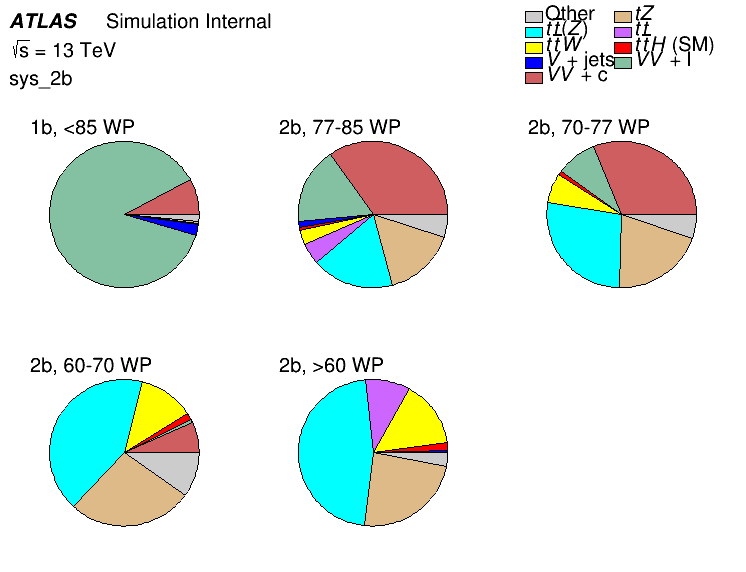
\includegraphics[width=0.7\linewidth]{sys_truthJets_2j/PieChart_postFit.png}
%    \caption{Post-fit background composition of the 2-jet fit regions.}
%    \label{fig:pie_chart_2j}
%\end{figure}


